



\begin{block}{Example}

\centering
\vspace{1cm}
    \heading{Updating with Observations and Predictions}
    \begin{equation*}
            \dciP \quad \vline \quad \dci
    \end{equation*}
    


\begin{columns}
\begin{column}{\textwidth}
    Hierarchical Bayes
    \begin{equation*}
    \Hbayes
    \end{equation*}
    
\end{column}
\begin{column}{\textwidth}
  Data Consistent Inversion  
    \begin{equation*}
           \dci
    \end{equation*}
\end{column}

\begin{column}{\textwidth}
  Simple Bayes
    \begin{equation*}
           \bayes
    \end{equation*}
\end{column}
\separatorcolumn
\end{columns}


\end{block}





\begin{block}{Takeaways}

\centering
\vspace{1cm}
    \heading{Data Consistent Inversion Performs Comparably with Hierarchical Bayes}
%     \begin{equation*}
%             \dciP \quad \vline \quad \dci
%     \end{equation*}
    %\begin{equation*}
    %        \dci
    %\end{equation*}
\begin{figure}
        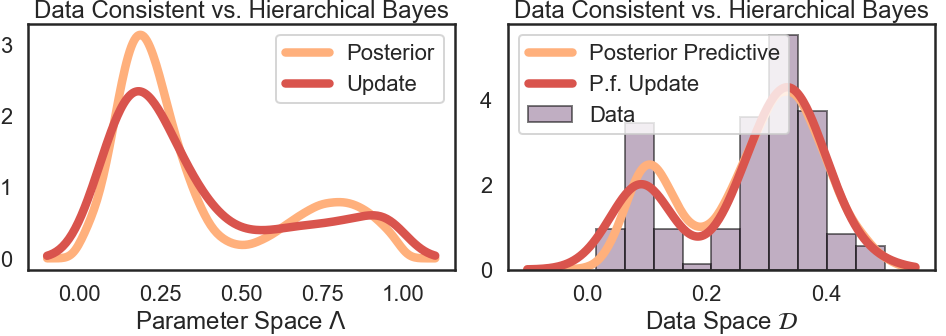
\includegraphics[width=30cm]{figures/distr_EX_comparison.png}
        \vspace{-0.5cm}
        \caption{ }
    \end{figure}
\end{block}
\heading{Non-parametric method with less sampling}
\heading{Future Research: How is it connected to Dirchlet Processes?}
